\section{A Tecnologia blockchain}
\subsection{Estrutura e funcionamento da blockchain}

\begin{frame}{Blockchain}
    \begin{block}{}
    \textbf{Blockchain} é o nome dado à tecnologia subjacente utilizada em diversas plataformas
    de gerenciamento descentralizado de posse de bens digitais baseada em \textbf{livro-razão distribuído}
    (do inglês, \textbf{\textit{Distributed Ledger Technology}} (DLT) )
    \end{block}
    Principais características:
    \begin{itemize}
        \item Armazenamento descentralizado e distribuído;
        \item Imutabilidade;
        \item Transparência;
        \item Dispensa da necessidade de confiança em uma terceira parte.
    \end{itemize}
       
\end{frame}

\begin{frame}{Blockchain Bitcoin}
    \begin{itemize}
        \item Primeiro caso de êxito: \textbf{Bitcoin};%\footnotemark[1];
            \item Criada em 2008 por Satoshi Nakamoto;
            \item Criptomoeda gerada e gerenciada de forma distribuída;
            \item Não possui entidades centralizadoras;
            \item Formada por uma rede de nós conectados auto-gerenciáveis;
            \item Nós trabalham para manter a integridade do sistema.
    \end{itemize}
    %\setcounter{footnote}{1}
    %\footcitetext{overview-bitcoin2008nakamoto}    
\end{frame}

\begin{frame}{Blockchain - Transações e blocos}
    \begin{itemize}
        \item Sempre que a posse de uma unidade ou fração de Bitcoin é transferida, uma \textbf{transação} é gerada;
        \item Quando uma nova transação ocorre, suas informações são transmitidas pela rede, tais como:
        \begin{itemize}
            \item Contas envolvidas;
            \item Quantia transferida;
            \item Assinatura digital;
            \item Horário da transação.
        \end{itemize}
        \item Os nós da rede, conhecidos como \textbf{mineradores}, coletam as transações e as armazenam em \textbf{blocos};
        \item Transações de um bloco são organizadas eu uma \textbf{árvore de Merkle}:
            \begin{itemize}
                \item Nós folhas: transações;
                \item Demais nós: Referências de \textit{hash}.
            \end{itemize}
    \end{itemize}
\end{frame}

\begin{frame}{Blockchain - Estrutura}
    \begin{figure}[!htb]
     \centering
     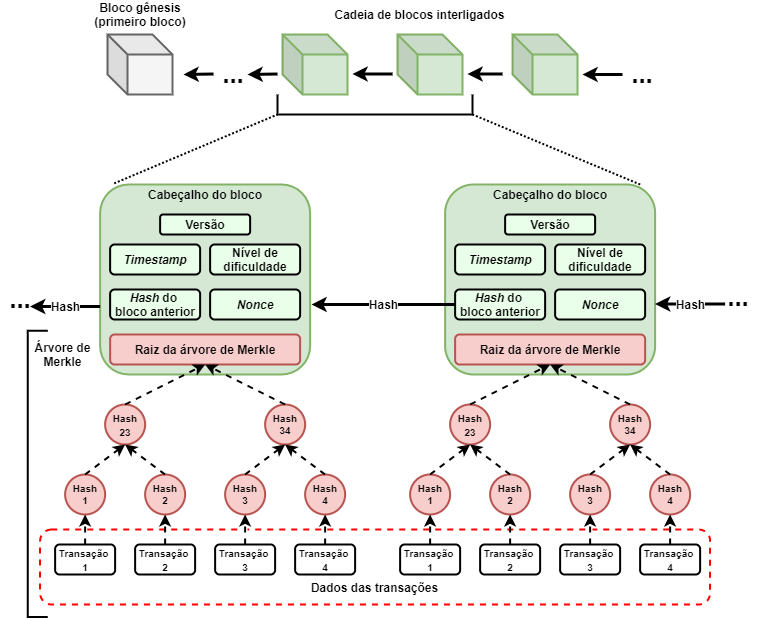
\includegraphics[scale=0.3]{figuras/blockchain/block_estrutura_cabeçalho.png}
    \end{figure}    
\end{frame}

\begin{frame}{Blockchain - Cabeçalho do bloco}
    \begin{enumerate}
        \item Versão;
        \item Hash do bloco anterior;
        \item Raiz da árvore de Merkle;
        \item \textit{Timestamp};
        \item Nível de dificuldade;
        \item \textit{nonce}.
    \end{enumerate}
    Criação do bloco:
    \begin{itemize}
        \item O minerador forma um bloco preliminar com os dados 1 ao 5;
        \item Por meio da resolução de um quebra-cabeça computacional, é obtido o \textit{nonce} do bloco;
        \begin{itemize}
            \item \textbf{Mineração} do bloco.
        \end{itemize}
        \item O \textit{nonce} é adicionado ao bloco;
        \item O bloco é transmitido pela rede.
    \end{itemize}
\end{frame}

\begin{frame}{Blockchain - Validação dos blocos}
    \begin{block}{}
    Para garantir a confiança de que os blocos na blockchain são legítimos, é necessário verificar a validade de um novo bloco antes deste ser inserido na rede.
    \end{block}
    \begin{block}{}
    Os nós são estimulados a manter a \textbf{integridade} das transações por meio de \textbf{mecanismos de incentivos}.
    \end{block}
\end{frame}

\begin{frame}{Blockchain - Validação dos blocos}
    \begin{block}{Algoritmo de consenso}
    \begin{itemize}
        \item Regras a serem seguidas pelos nós para criação e validação dos blocos;
        \item Recompensa para os nós honestos;
        \item Garante que todos os nós da rede concordem com o histórico de transações que compõem os blocos da blockchain;
    \end{itemize}
    \end{block}    
\end{frame}

\begin{frame}{Blockchain - Algoritmos de consenso}
    \begin{exampleblock}{\textit{Proof-of-Work} (PoW)}
    \begin{itemize}
        \item Utilizado nas blockchains Bitcoin e Ethereum;
        \item Consiste na competição entre os mineradores para resolução do \textit{nonce} do bloco;
        \item O vencedor transmite o bloco pela rede para validação;
        \item Quanto maior o poder computacional do minerador, maior a chance de vencer;
        \item Resulta em um alto esforço computacional e gasto energético;
        \item O vencedor receber um valor da criptomoeda como recompensa (e.g., Bitcoin);
        \item \textbf{Desvantagem}: Esforço computacional elevado.
    \end{itemize}
    \end{exampleblock}
\end{frame}

\begin{frame}{Blockchain - Algoritmos de consenso}
    \begin{exampleblock}{\textit{Proof-of-Stake}(PoS)}
    \begin{itemize}
        \item Nós \textbf{validadores} participam da criação dos blocos;
        \item Validadores investem um \textbf{valor de participação};
        \item Quanto maior o valor, maior a chance de ser escolhido para validar o próximo bloco;
        \item Ethereum 2.0: migração para o protocolo PoS.
    \end{itemize}
    \end{exampleblock}
\end{frame}

\begin{frame}{Blockchain - Algoritmos de consenso}
    \begin{exampleblock}{\textit{Practical Byzantine Fault Tolerance}(PBFT)}
    \begin{itemize}
        \item Há dois tipos de nós: \textbf{cliente} e \textbf{servidor};
        \item Um nó cliente envia um bloco aos nós servidores;
        \item Se o bloco for validado por um número suficiente de nós, então é adicionado à blockchain;
        \item Utilizado na blockchain \textit{Hyperledger Fabric}.
    \end{itemize}
    \end{exampleblock}     
\end{frame}

\begin{frame}{Blockchain - Escolha do histórico de transações}
    \begin{itemize}
    \item O trabalho dos mineradores consiste na alternação de duas tarefas:
    \begin{itemize}
        \item Analisar a validade de um novo bloco;
        \item Criar o próximo bloco.
    \end{itemize}
    \item A transmissão e entrega de novos blocos sobrem influências externas;
    \item Assim, nós da rede podem ter informações distintas à sua disposição ao mesmo tempo;
    \item Quando um nó recebe mais de um nó com o mesmo bloco pai, é criado um \textit{fork};
    \end{itemize}
\end{frame}

\begin{frame}{Blockchain - Escolha do histórico de transações}
    \begin{itemize}
        \item Na Bitcoin, a \textbf{cadeia mais longa} é escolhida;
        \item A ramificação escolhida pela maioria dos nós é considerada a \textbf{cadeia de blocos principal}.
    \end{itemize}
    \begin{figure}[!htb]
    \centering
    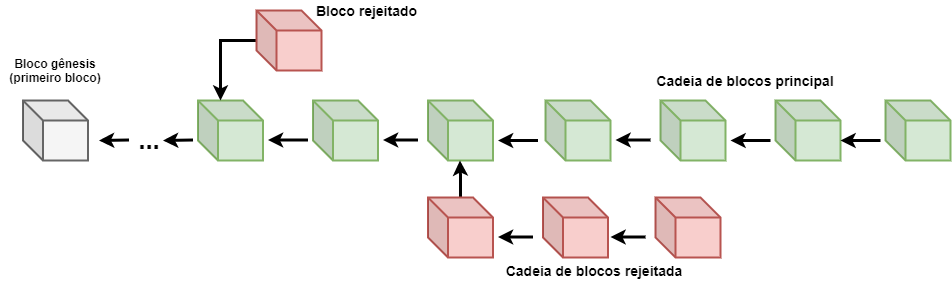
\includegraphics[scale=0.3]{figuras/blockchain/cadeia_de_blocos.png}
    \end{figure}    
\end{frame}

\begin{frame}{Blockchain - Criptografia e autorização de transações}
    \begin{itemize}
        \item Um dos pilares da blockchain consiste na \textbf{segurança} e \textbf{integridade} das transações;
        \item Apenas o proprietário legítimo pode realizar a transferência de uma criptomoeda para outra conta;
        \item Para isso, é utilizada uma \textbf{assinatura digital};
        \begin{itemize}
            \item Criptografia assimétrica;
            \item Chaves pública e privada.
        \end{itemize}
        \item A assinatura é utilizada na \textbf{assinatura} e na \textbf{verificação} de uma transação.
    \end{itemize}
\end{frame}

\begin{frame}{Blockchain - Criptografia e autorização de transações}
    \begin{itemize}
        \item \textbf{Assinatura:}
    \end{itemize}
    \begin{figure}[!htb]
     \centering
     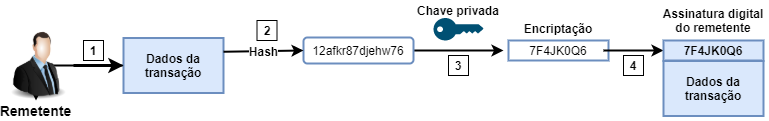
\includegraphics[scale=0.4]{figuras/blockchain/remetente_assinatura_digital.png}
    \end{figure}
    \begin{itemize}
        \item \textbf{Verificação:}
    \end{itemize}    
    \begin{figure}[!htb]
     \centering
     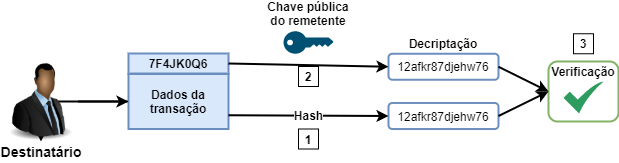
\includegraphics[scale=0.4]{figuras/blockchain/verifica_assinatura_digital.png}
    \end{figure}
\end{frame} 

% no final da explicação de blockchain, fazer um slide falando pq é difícil fraudar um bloco

\subsection{Blockchain Ethereum}

\begin{frame}{Ethereum}
    \begin{block}{}
    \begin{itemize}
        \item Apesar da blockchain ter sido criada para uma aplicação financeira (i.e., a Bitcoin), seus conceitos e protocolos podem ser estendidos para diversas áreas;
        \item É apenas um fim para um meio;
    \end{itemize}
    \end{block}
    \begin{block}{}
    \begin{itemize}
        \item Em 2014 foi criada a blockchain \textbf{Ethereum};
        \item Introdução dos contratos inteligentes;
        \item Pioneira na expansão das aplicações da blockchain.
    \end{itemize}
    \end{block}
\end{frame}

\begin{frame}{Ethereum}
    \begin{itemize}
        \item Definida como uma plataforma de computação \textbf{distribuída} composta por uma rede de computadores que operam de forma \textbf{descentralizada}, \textbf{autônoma} e \textbf{democrática};
        \item Permite a geração, transferência e gerenciamento de sua criptomoeda, o \textbf{Ether};
        \item Seu funcionamento é baseado na implantação da \textbf{contratos inteligentes} (CI):
        \begin{itemize}
            \item Programas de computador;
            \item Executam automatica e obrigatoriamente aquilo que foi programado;
            \item Estabelecem um acordo entre os envolvidos;
            \item Quando compilado, é convertido em \textit{bytecode};
            \item Executado na Máquina Virtual Ethereum (MVE);
            \item Geração de transações.
        \end{itemize}
    \end{itemize}
\end{frame} 

\begin{frame}{Ethereum}
    \begin{itemize}
        \item Transações são coletadas e estruturadas nos blocos em uma \textit{trie};
        \item Opera de forma semelhante à Bitcoin na garantia da \textbf{imutabilidade};
        \item Aplicações Descentralizadas (do inglês, \textit{Descentralized Applications} (DApps)):
        \begin{itemize}
            \item Mais de 3 mil utilizam a Ethereum~\footnote{\url{<https://www.stateofthedapps.com/>}}.
        \end{itemize}
        \item Em 2021, seu valor de mercado superou \$400 bilhões~\footnote{<https://coinmarketcap.com/>};
        \item Há ao menos 2 milhões de CIs já executados~\footnote{<https://etherscan.io/>}.
    \end{itemize}
\end{frame}

\begin{frame}{Ethereum - Propriedades}
    As aplicações que executam sobre a Ethereum dispõem de uma série de propriedades:
    \begin{itemize}
        \item Descentralização;
        \item Imutabilidade;
        \item Persistência de dados;
        \item Execução autônoma;
        \item Acurácia.
    \end{itemize}
\end{frame}

\begin{frame}{Ethereum - Contas}
    Dois tipos:
    \begin{itemize}
        \item Conta de Propriedade Externa (CPE):
        \begin{itemize}
            \item Armazena os fundos dos usuários em Wei (1 Ether = 10$^{18}$ Wei);
            \item Associadas e controladas por uma chave privada.
        \end{itemize}
        \item Conta de contrato (CC):
        \begin{itemize}
            \item Conta associada à um CI;
            \item Controladas pelo código de um \textit{bytecode} executável.
        \end{itemize}
    \end{itemize}
\end{frame}

\begin{frame}{Ethereum - Contas e mensagens}
Contas:
    \begin{itemize}
        \item Estado global da Ethereum = estado de todas as contas;
        \item Estado dinâmico definido por:
        \begin{itemize}
            \item \textit{nonce:}
            \begin{itemize}
                \item CPE: transações iniciadas pelo proprietário;
                \item CC: contratos criados pela conta.
            \end{itemize}
            \item \textit{balance:} saldo em Wei da CPE ou CC;
            \item \textit{storageRoot:} CC - \textit{Hash} da raiz da \textit{trie};
            \item \textit{codeHash:} \textit{Hash} do \textit{bytecode} da CC correspondente.
        \end{itemize}
    \end{itemize}
Mensagem: 
    \begin{itemize}
        \item Meio de interação CPE -> CC e CPE -> CPE;
        \item Especifica uma instrução a ser executada;
        \item Usadas para transferência de Ether e execução de CIs;
        \item Sempre que uma CC recebe uma mensagem seu código é ativado
    \end{itemize}    
\end{frame}

\begin{frame}{Ethereum - Transações e transição de estados}
Transação: 
    \begin{itemize}
        \item Pacote de dados que armazena uma mensagem;
        \item Execução resultado em um custo computacional (\textit{gas});
        \item \textit{gasPrice:} custo, em Wei, por unidade de \textit{gas};
        \item Quanto maior o \textit{gasPrice}, maior a recompensa para o minerador;
        \item \textit{gasLimit:}
        \begin{itemize}
            \item Evita o consumo indefinido de \textit{gas}.
        \end{itemize}
    \end{itemize}
Transição de estados:
    \begin{itemize}
        \item Quando uma transação é executada, algum atributo de alguma conta é alterado.
        \begin{itemize}
            \item Ex: saldo da conta ou variável de um CI.
        \end{itemize}
        \item Transição: $(S, TX)\longrightarrow S'$.
    \end{itemize}
\end{frame}

\begin{frame}{Ethereum - Formação dos blocos}
    \begin{itemize}
        \item Transações são transmitidas pela rede;
        \item Mineradores possuem uma \textit{pool} de transações pendentes;
        \item Transações da \textit{pool} são escolhidas para formar os blocos.
    \end{itemize}
    \begin{figure}[!htb]
     \centering
     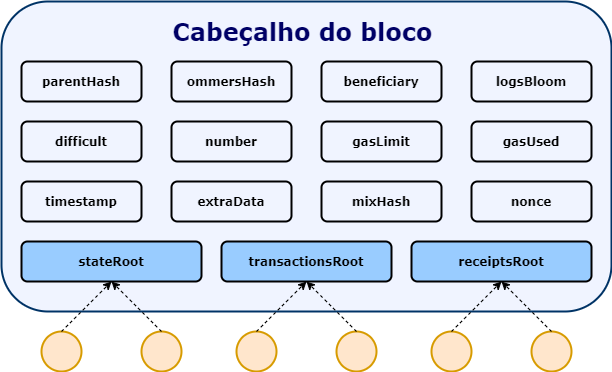
\includegraphics[scale=0.3]{figuras/blockchain/eth_block_header.png}
    \end{figure}    
\end{frame}

\begin{frame}{Ethereum - Validação}
    \begin{itemize}
        \item Na Ethereum podem ocorrer \textit{forks} com versões distintas do histórico de transações;
        \item Cadeia principal: aquela com a maior dificuldade acumulada.
    \end{itemize}
    \begin{figure}[!htb]
     \centering
     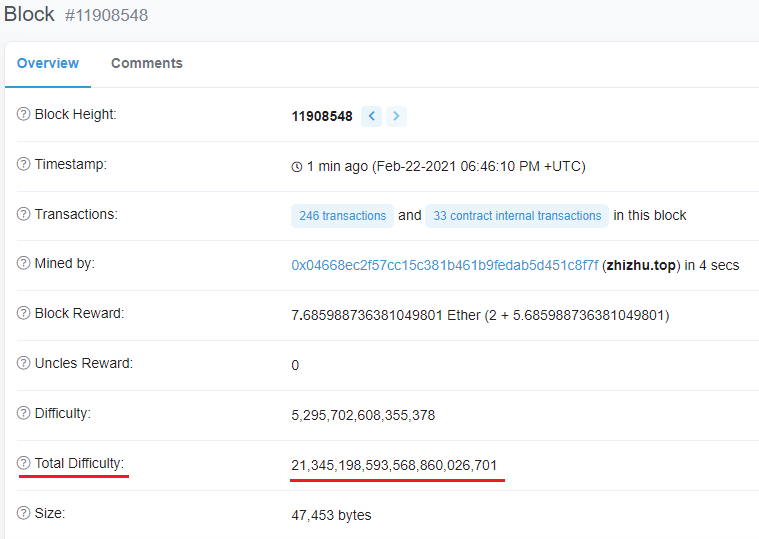
\includegraphics[scale=0.35]{figuras/blockchain/block-eth-difficulty.png}
    \end{figure} 
\end{frame}

\begin{frame}{Blockchain - Estágios evolutivos}
    \begin{block}{}
    Após o êxito da Bitcoin, outras criptomoedas e tecnologias baseadas na blockchain foram desenvolvidas.
    \end{block}
    Esses avanços são classificados como:
    \begin{itemize}
        \item Blockchain 1.0 (Bitcoin):
        \begin{itemize}
            \item Geração e gerenciamento de criptomoedas.
        \end{itemize}
        \item Blockchain 2.0 (Ethereum):
        \begin{itemize}
            \item Junção entre CIs e criptomoedas;
            \item Aplicações financeiras;
            \item Ex: DApps, Organizações Autônomas Descentralizadas (OADs).
        \end{itemize}
        \item Blockchain 3.0:
        \begin{itemize}
            \item Aplicações em outras áreas além da financeira;
            \item Ex: Cuidados médicos, inteligência artificial, internet das coisas, governança descentralizada, entre outras.
        \end{itemize}
    \end{itemize}
\end{frame}

\begin{frame}{Ethereum - Aplicações}
    \begin{itemize}
        \item Sistema de \textbf{tokens}:
        \begin{itemize}
            \item Tokenização;
            \item \textit{Stable coins}: Tether, USD Coin, Pax Gold;
            \item Padrão ERC-20.
        \end{itemize}
        \item Organização Autônoma Descentralizada:
        \begin{itemize}
            \item Regras operacionais e de gerenciamento são programadas em um CI;
            \item Abolição de modelos baseados em hierarquia;
            \item Redução de custos;
            \item Primeira OAD: \textit{The DAO}.
        \end{itemize}
        \item Cuidados métodos e serviços de saúde:
        \begin{itemize}
            \item Integração de dados de prontuários.
        \end{itemize}
    \end{itemize}
\end{frame}

\begin{frame}{Ethereum - Arquitetura em camadas}
    \begin{figure}[!htb]
     \centering
     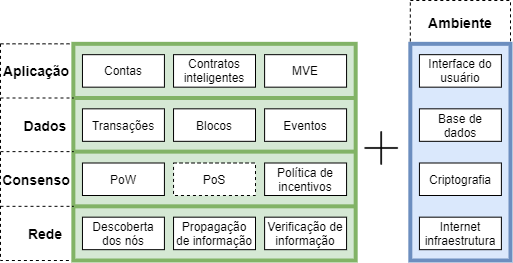
\includegraphics[scale=0.5]{figuras/blockchain/ethereum_arquitetura.png}
    \end{figure}    
\end{frame}